\parindent=0em
\subsection{DAQRI Smart Helmet}
\noindent

%https://www.linkedin.com/pulse/daqri-smart-helmet-closer-look-nathan-gaydhani

El \textit{DAQRI Smart Helmet} es un \textit{HMD} enfocado al uso industrial, está formado por un dispositivo de realidad mixta sin cables integrado en un casco duro (cascos utilizados por ejemplo en la construcción). Ya que está pensado para un uso industrial está dotado de 4 cámaras para poder capturar todo el entorno, es decir, abarcar 360º.\\

Con el objetivo de proteger al usuario en entornos industriales peligrosos, el dispositivo cuenta con una cámara termográfica (para poder controlar lugares potencialmente peligrosos debido a su temperatura) y barómetro para poder medir la presión del entorno.\\

Para el seguimiento, el \textit{DAQRI Smart Helmet} utiliza la tecnología \textit{SLAM} y posee \textit{6DoF} para el movimiento y los giros del usuario. Del mismo modo, ya que el objetivo final es proteger al usuario, el dispositivo cuenta con reconocimiento de órdenes por voz y de control de movimientos de la cabeza para manejar el \textit{HMD}, de esta forma se pueden tener las manos libres.\\

\begin{figure}[h]
    \centering
    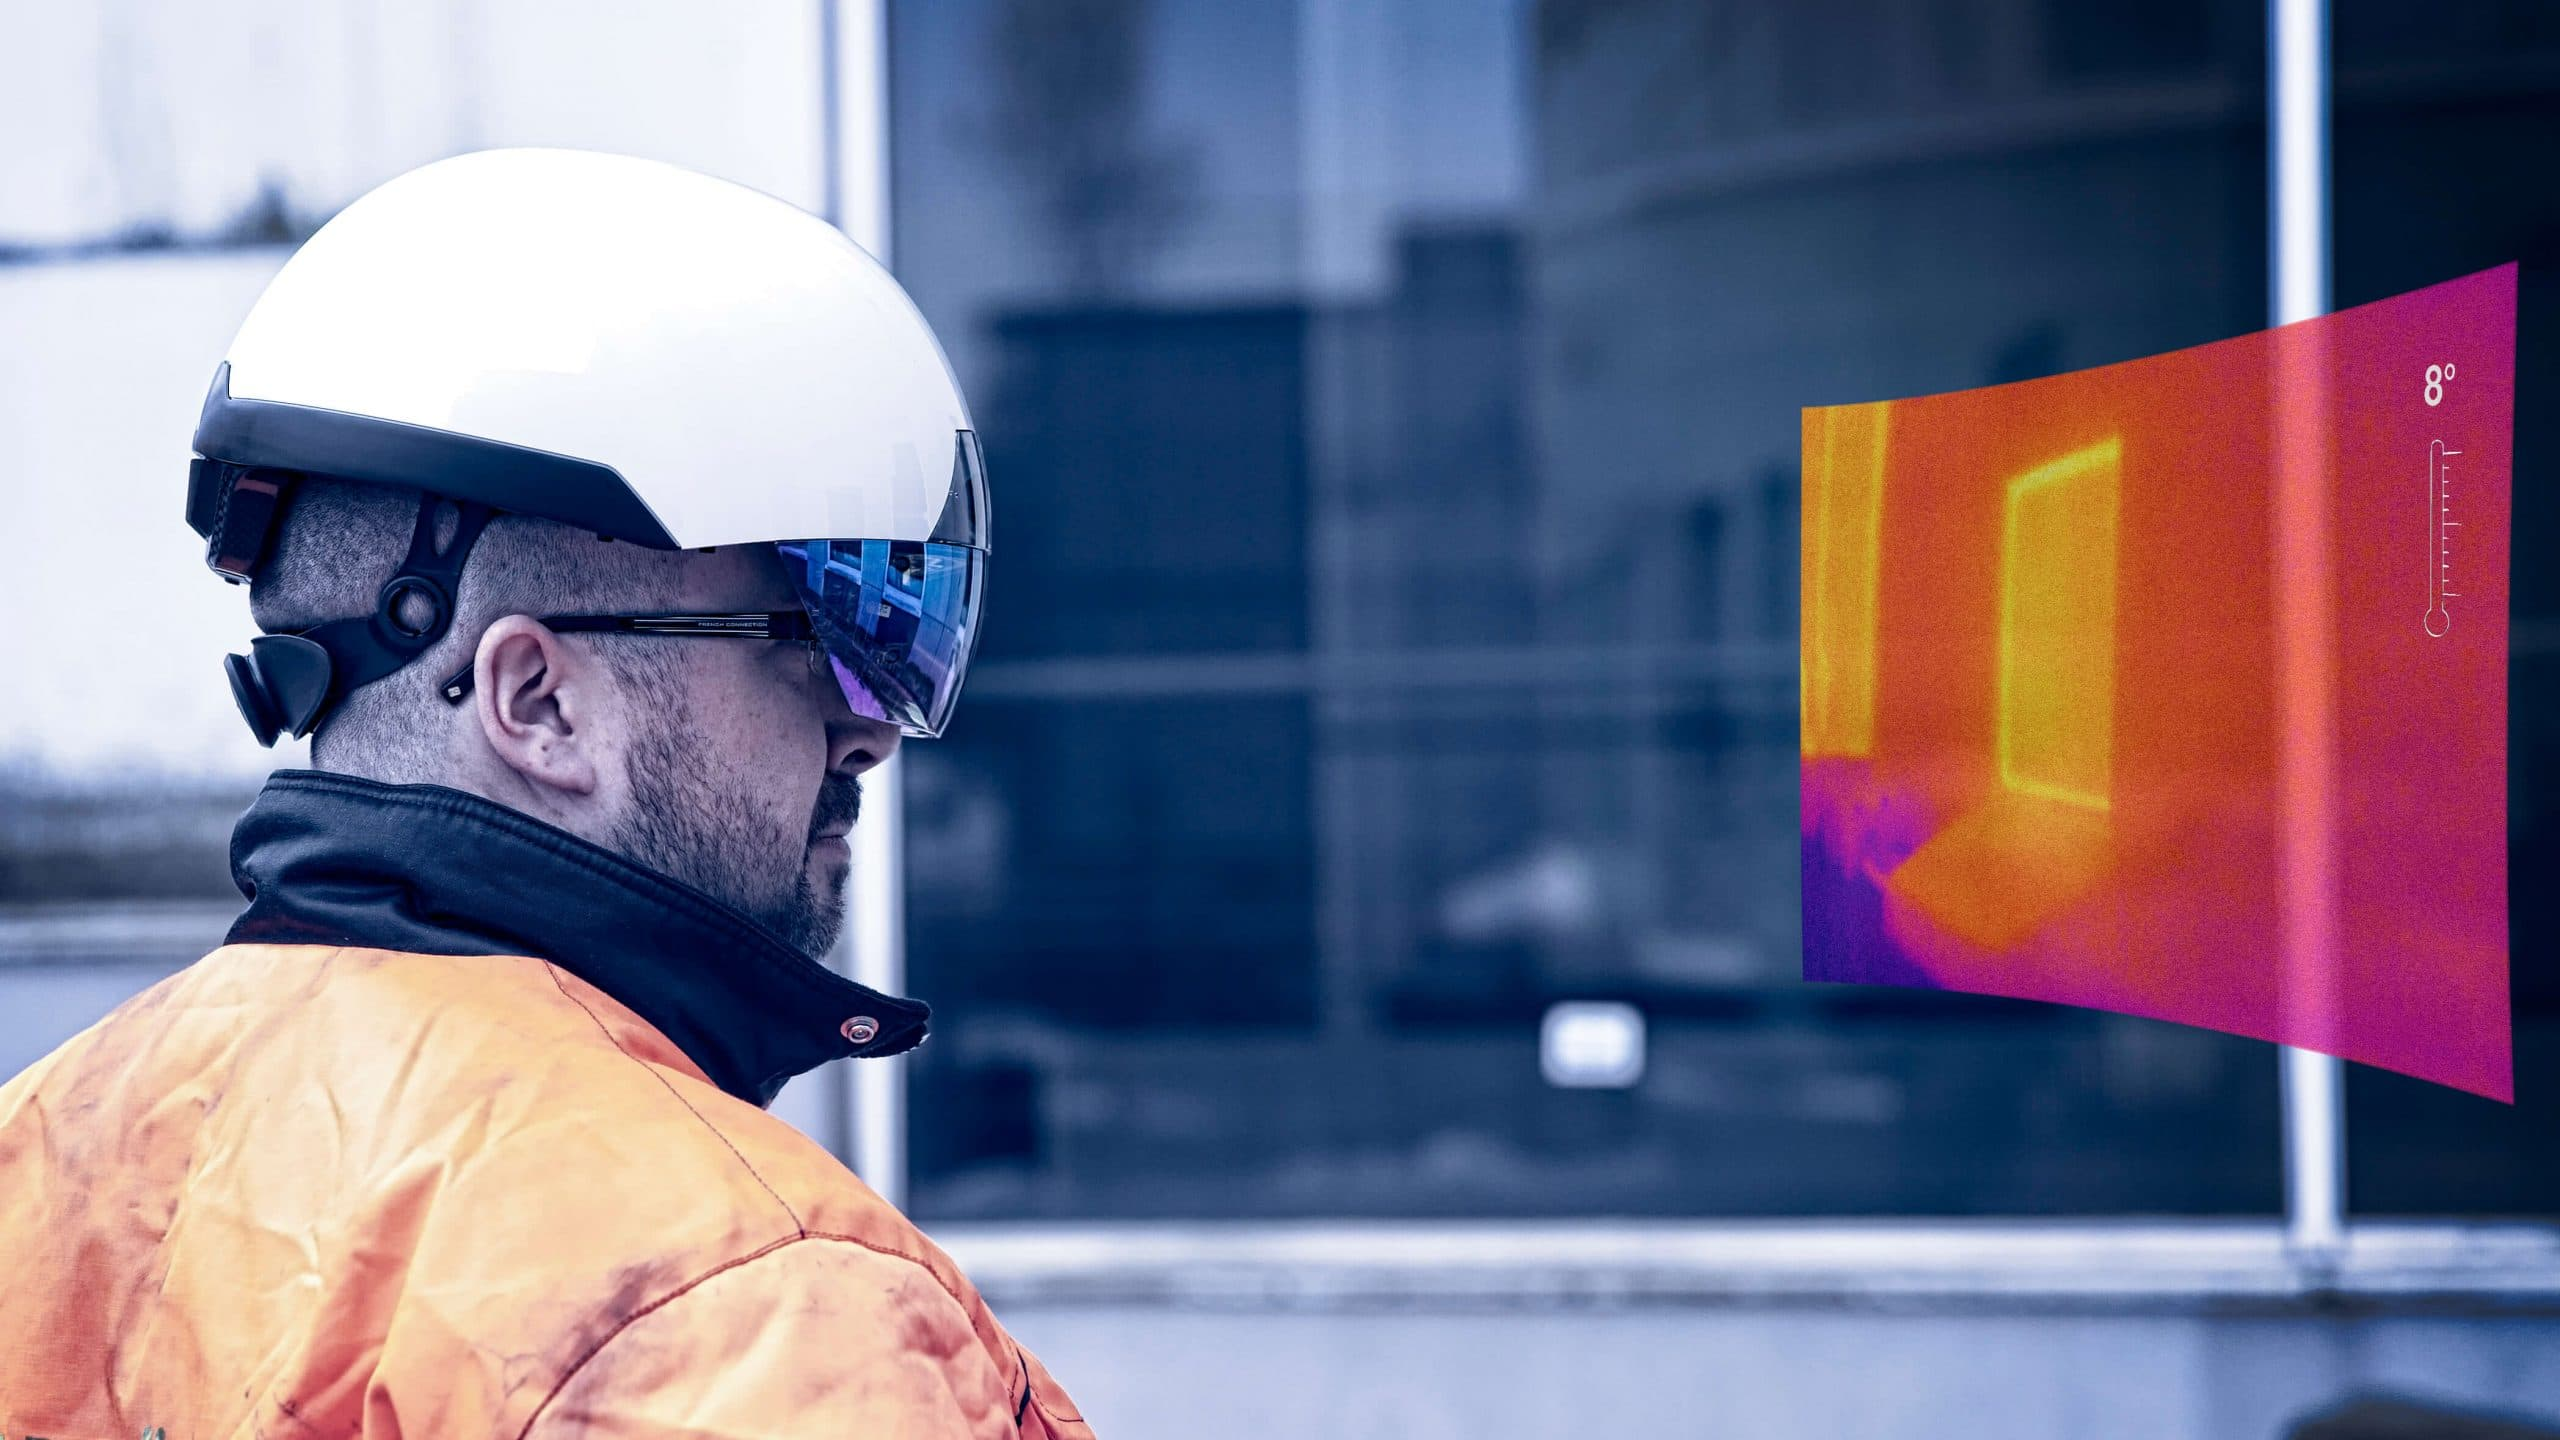
\includegraphics[scale=0.12]{Images/Estado del arte/daqrihelmet.jpg}
    \caption{Vista del DAQRI Smart Helmet}
    \label{fig:vistaDAQRIHelmet}
\end{figure}

Finalmente, cabe recalcar que el casco goza de procesadores y un sistema operativo \textit{Android} para ser totalmente independiente, también, utiliza unas baterías intercambiables de 5700 miliamperios por hora y dispone de conectividad \textit{WiFi} para poder comunicarse por vídeo en tiempo real remotamente con otros usuarios. El casco tiene un peso total de 1 kilo y~500 gramos y su precio actual es de~15.000 dólares.

%\footnotetext{\label{daqriImagefooter}{Imagenes obtenida de: %\url{https://www.stereoscape.com/blog/2017/04/25/daqri-smart-helmet-so-m%uch-more-than-a-helmet/}.}}


